\section{FAC-ECL Family}

The third model family implemented in this project is Frequency-Aware Exposure-Consistent Low-Light Enhancement (FAC-ECL). This family is introduced after the illumination-guided U-Net because the previous experiment showed that providing an explicit brightness cue is useful but not sufficient. In particular, the illumination-guided model reduced some residual darkness indicators, but it did not consistently improve full-reference reconstruction and still showed color imbalance, texture loss, residual noise, and local artifacts.

FAC-ECL tests a different hypothesis. Instead of adding another input channel, it keeps the image representation unchanged and modifies the training objective. The motivation is that low-light enhancement errors do not all have the same visual nature. Exposure and color errors usually affect large and smooth image regions, while texture, noise, edges, and halo artifacts are local high-frequency phenomena. Therefore, this family tries to separate these aspects during training. The idea is related to frequency-aware reconstruction objectives~\cite{DBLP:conf/iccv/JiangDWL21}, exposure-oriented low-light enhancement losses~\cite{DBLP:conf/cvpr/GuoLGLHKC20}, and Retinex or degradation-aware methods that distinguish illumination-related effects from reflectance or degradation-related effects~\cite{DBLP:conf/bmvc/WeiWY018, DBLP:journals/dsp/WeiLL24}. However, in this work FAC-ECL is implemented as a lightweight training-objective variant of the U-Net baseline, rather than as a full Retinex decomposition model.

\subsection{Architecture}

FAC-ECL relies on the same U-Net backbone as the two preceding variants, while keeping the output unchanged: the network predicts a three-channel enhanced RGB image.

Unlike the illumination-guided U-Net, FAC-ECL does not concatenate an illumination map to the input, that remains a standard three-channel RGB low-light image. This is an important design choice because the purpose of FAC-ECL is not to test a different input representation, but to test a different supervision strategy with additional constraints that distinguish illumination, color, detail, and stability.

For this reason, the architectural hyperparameters that are not specific to FAC-ECL are fixed to the best configuration selected for the classical U-Net family. This choice is more appropriate than inheriting the best configuration of the illumination-guided U-Net, because FAC-ECL uses a three-channel input, while the illumination-guided model uses a four-channel input. Keeping the same backbone also makes the comparison easier to interpret: any difference between the baseline U-Net and FAC-ECL is mainly due to the training objective, not to a different model capacity or input format.

During normal inference, FAC-ECL behaves exactly like the classical U-Net: one low-light RGB image is given as input, and one enhanced RGB image is produced. The extra mechanism is used only during training. In this phase, the wrapper creates two versions of the same input: the original image and a mildly perturbed copy, obtained with small photometric changes such as exposure, gamma, color, or noise variations.

The original input produces the main output. This output is compared with the paired target through the reconstruction loss and the frequency-aware losses, so it teaches the model what the enhanced image should look like. The perturbed input is passed through the same U-Net, with the same weights, and its output is compared only with the main output. This gives the exposure-consistency loss. In this way, the same network learns both to match the target and to remain stable when the low-light input changes slightly.

\subsection{Training Objective and Grid Search}

FAC-ECL follows the same experimental protocol used for the previous model families, but it changes the training objective. The classical U-Net and the illumination-guided U-Net are trained with a direct L1-SSIM reconstruction loss. FAC-ECL keeps this reconstruction term, because the task is still paired image enhancement, but adds two additional constraints. The first one is frequency-aware supervision, which separates smooth illumination and color information from local detail information. The second one is exposure consistency, which encourages the model to produce stable outputs when the same low-light image is slightly modified.

The frequency-aware part separates each image into a low-frequency component and a high-frequency component. The low-frequency component is obtained by applying a Gaussian blur to the image:
\begin{equation}
	\mathrm{Low}(I;\sigma)
	=
	G_{\sigma} \ast I,
	\label{eq:fac_ecl_low_frequency}
\end{equation}
where $I$ is the RGB image to be decomposed, $G_{\sigma}$ is a Gaussian kernel with standard deviation $\sigma$, and $\ast$ denotes convolution. The term $\mathrm{Low}(I;\sigma)$ therefore represents the smoothed version of image $I$ obtained by convolving it with the Gaussian kernel $G_{\sigma}$. The parameter $\sigma$ controls the strength of the smoothing: a larger value produces a stronger blur, while a smaller value keeps the smoothing more local. This low-frequency component contains smooth information such as global illumination, broad exposure changes, and slowly varying color trends.

The high-frequency component is computed as the residual between the original image and its low-frequency version:
\begin{equation}
	\mathrm{High}(I;\sigma)
	=
	I - \mathrm{Low}(I;\sigma).
	\label{eq:fac_ecl_high_frequency}
\end{equation}
Here, $\mathrm{High}(I;\sigma)$ is the high-frequency component of image $I$ computed using the same smoothing parameter $\sigma$. It represents what remains after subtracting the smooth component from the original image, and therefore mainly contains rapid spatial variations such as local details, edges, texture, noise, and fine artifacts.

The exposure-consistency term is used to make the model more stable. During training, FAC-ECL takes the same low-light input image and creates a slightly modified version of it. This modified version is obtained with mild photometric changes, such as a small change in exposure, a small gamma correction, a slight color-temperature shift, or a small amount of low-light noise. The scene does not change: the objects, the structure, and the content of the image are still the same. Only the low-light appearance is slightly different. Therefore, the enhanced outputs should also be similar. If the model produces very different enhanced images from these two similar inputs, its prediction is not stable. For this reason, FAC-ECL adds a penalty between the output produced from the original input and the output produced from the perturbed input.

The complete objective is defined by combining four terms. The first one is the reconstruction loss, which is the same L1-SSIM objective used for the previous U-Net families:
\begin{equation}
	\mathcal{L}_{\mathrm{rec}}
	=
	0.8\,\mathrm{MAE}(\hat{I}, I)
	+
	0.2\,\bigl(1-\mathrm{SSIM}(\hat{I}, I)\bigr).
	\label{eq:fac_ecl_rec_loss}
\end{equation}
Here, $\hat{I}$ is the enhanced image predicted by the model, while $I$ is the paired normally exposed target. The MAE term penalizes pixel-wise differences, whereas the SSIM term encourages structural similarity between prediction and target.

The second and third terms apply the same idea to the frequency decomposition introduced above. The low-frequency term compares the smooth components of prediction and target, while the high-frequency term compares their residual detail components:
\begin{equation}
	\mathcal{L}_{\mathrm{low}}
	=
	\mathrm{MAE}
	\bigl(
	\mathrm{Low}(\hat{I};\sigma),
	\mathrm{Low}(I;\sigma)
	\bigr),
	\label{eq:fac_ecl_low_loss}
\end{equation}
\begin{equation}
	\mathcal{L}_{\mathrm{high}}
	=
	\mathrm{MAE}
	\bigl(
	\mathrm{High}(\hat{I};\sigma),
	\mathrm{High}(I;\sigma)
	\bigr).
	\label{eq:fac_ecl_high_loss}
\end{equation}
The low-frequency loss is intended to guide broad illumination, exposure, and color correction, while the high-frequency loss focuses on local structures such as edges, texture, and fine details.

The fourth term is the exposure-consistency loss. It compares the prediction obtained from the original low-light input with the prediction obtained from a mildly perturbed version of the same input:
\begin{equation}
	\mathcal{L}_{\mathrm{cons}}
	=
	\mathrm{MAE}
	\bigl(
	f(x),
	f(T(x))
	\bigr).
	\label{eq:fac_ecl_cons_loss}
\end{equation}
In this equation, $x$ is the original low-light input, $T(x)$ is the same input after a mild photometric perturbation, and $f$ is the enhancement network. Since both inputs represent the same scene, this term encourages the model to produce similar enhanced outputs instead of reacting too strongly to small exposure, gamma, color, or noise variations.

The final FAC-ECL objective is obtained by weighting and summing these components:
\begin{equation}
	\begin{aligned}
		\mathcal{L}_{\mathrm{FAC\text{-}ECL}}
		&=
		\mathcal{L}_{\mathrm{rec}}
		+
		\lambda_{\mathrm{low}}\,\mathcal{L}_{\mathrm{low}} \\
		&\quad+
		\lambda_{\mathrm{high}}\,\mathcal{L}_{\mathrm{high}}
		+
		\lambda_{\mathrm{cons}}\,\mathcal{L}_{\mathrm{cons}}.
	\end{aligned}
	\label{eq:fac_ecl_loss}
\end{equation}
The coefficients $\lambda_{\mathrm{low}}$, $\lambda_{\mathrm{high}}$, and $\lambda_{\mathrm{cons}}$ control the importance of the low-frequency, high-frequency, and consistency terms, respectively.

The FAC-ECL grid search is designed to keep the comparison with the previous families controlled. Since FAC-ECL still uses a standard three-channel RGB input, the closest architectural reference is the best configuration selected for the classical U-Net family, not the illumination-guided U-Net. Therefore, the channel schedule, normalization strategy, upsampling method, and weight decay are fixed to the selected classical U-Net values.

The learning rate is still varied in the grid. This is necessary because FAC-ECL changes the objective optimized during training. Adding low-frequency, high-frequency, and consistency terms can change the magnitude and direction of the gradients. If the learning rate were fixed, a poor result could be caused by an unsuitable optimization scale rather than by the FAC-ECL idea itself. For this reason, the grid includes the learning rate together with the FAC-ECL-specific loss weights. The explored hyperparameter space is:

\begin{itemize}[topsep=5pt]
	\item Learning rate $\in$ $2{\cdot}10^{-4}$, $3{\cdot}10^{-4}$, $5{\cdot}10^{-4}$, $10^{-3}$;
	\item Low-frequency weight $\lambda_{\mathrm{low}} \in$ $0.05$, $0.10$, $0.20$;
	\item High-frequency weight $\lambda_{\mathrm{high}} \in$ $0.05$, $0.10$, $0.20$;
	\item Exposure-consistency weight $\lambda_{\mathrm{cons}} \in$ $0.02$, $0.05$, $0.10$, $0.20$.
\end{itemize}

The low-frequency weight controls how strongly the model is encouraged to match the smooth illumination and color structure of the target. If this value is too small, the model may behave similarly to the classical U-Net and may not sufficiently address exposure or color errors. If it is too large, the model may over-prioritize smooth brightness and color trends at the expense of local detail.

The high-frequency weight controls how strongly the model is encouraged to match local structures. This term is intended to reduce over-smoothing and preserve edges and texture. However, it must be balanced carefully because high-frequency content can also include noise, especially in very dark regions.

The exposure-consistency weight controls the importance of stability under photometric perturbations. A small value makes the consistency term a weak regularizer, while a larger value forces the model to produce more similar outputs for the original and perturbed inputs. This can improve robustness, but an excessive value may also make the model too conservative and reduce its ability to adapt to difficult low-light inputs.

The Gaussian blur used for the frequency decomposition is kept fixed in the grid, with kernel size $15 \times 15$ and standard deviation $\sigma = 3.0$. These values are chosen to separate broad illumination and color trends from local texture and edge information. The photometric perturbation ranges are also fixed and kept mild, because the goal is not to create a new synthetic dataset, but to expose the model to small realistic variations of the same input scene.

Combining these choices gives 144 FAC-ECL configurations in the single-seed screening stage.

\subsection{Quantitative Analysis}

This subsection reports the quantitative behavior of the selected FAC-ECL family. The final configuration is the one selected by the fixed experimental protocol of this project, and has $1.93$M trainable parameters. Table~\ref{tab:fac_ecl_final_evaluation} reports the final evaluation of the selected FAC-ECL configuration.

\begin{table*}[t]
	\centering
	\caption{Final evaluation of the selected FAC-ECL configuration. The first row reports the in-domain evaluation, while the remaining rows report cross-dataset evaluation results. Values are reported as mean $\pm$ standard deviation across three seeds. Full-reference metrics are not available for ExDark because it is unpaired.}
	\label{tab:fac_ecl_final_evaluation}
	\resizebox{\textwidth}{!}{
		\begin{tabular}{lccccccccccc}
			\toprule
			Dataset & SSIM & PSNR (dB) & MAE & NIQE & BRISQUE & Mean $Y$ & Std $Y$ & Dark (\%) & Clip (\%) & RGBI & Lap. sharp. \\
			\midrule
			LOL-v2 Real & $0.851 \pm 0.007$ & $19.85 \pm 0.39$ & $0.101 \pm 0.004$ & $6.59 \pm 0.02$ & $28.53 \pm 3.83$ & $0.455 \pm 0.008$ & $0.164 \pm 0.004$ & $1.4 \pm 0.1$ & $0.08 \pm 0.02$ & $0.037 \pm 0.002$ & $0.0091 \pm 0.0003$ \\
			\midrule
			LOL-v2 Synthetic & $0.763 \pm 0.004$ & $17.32 \pm 0.08$ & $0.126 \pm 0.002$ & $7.13 \pm 0.02$ & $33.47 \pm 1.76$ & $0.441 \pm 0.007$ & $0.209 \pm 0.007$ & $2.8 \pm 0.7$ & $0.10 \pm 0.05$ & $0.038 \pm 0.002$ & $0.0093 \pm 0.0009$ \\
			LOL-v1 & $0.886 \pm 0.004$ & $22.13 \pm 0.41$ & $0.076 \pm 0.004$ & $6.70 \pm 0.06$ & $29.96 \pm 3.62$ & $0.465 \pm 0.010$ & $0.178 \pm 0.005$ & $2.6 \pm 0.2$ & $0.05 \pm 0.02$ & $0.050 \pm 0.003$ & $0.0086 \pm 0.0003$ \\
			MILLs & $0.777 \pm 0.010$ & $18.00 \pm 0.22$ & $0.119 \pm 0.004$ & $6.15 \pm 0.31$ & $22.66 \pm 5.48$ & $0.428 \pm 0.011$ & $0.121 \pm 0.003$ & $1.4 \pm 0.5$ & $0.00 \pm 0.00$ & $0.082 \pm 0.010$ & $0.0057 \pm 0.0003$ \\
			ExDark & -- & -- & -- & $7.01 \pm 0.08$ & $34.83 \pm 2.96$ & $0.398 \pm 0.007$ & $0.195 \pm 0.003$ & $4.4 \pm 1.0$ & $0.12 \pm 0.05$ & $0.073 \pm 0.002$ & $0.0078 \pm 0.0009$ \\

			\bottomrule
		\end{tabular}
	}
\end{table*}

\analysispar{In-domain and cross-dataset evaluation}
LOL-v2 Real remains the in-domain reference, because it comes from the same real-captured dataset used for training and validation. On this dataset, FAC-ECL obtains $0.851$ SSIM, $19.85$ dB PSNR, and $0.101$ MAE. These values are slightly better than the corresponding results of the baseline U-Net and of the illumination-guided U-Net. This indicates that the frequency-aware and exposure-consistency terms do not damage the source-domain reconstruction. On the contrary, they help the same U-Net backbone produce outputs that are a little closer to the paired target.

LOL-v1 is again the closest cross-dataset case. FAC-ECL obtains $0.886$ SSIM, $22.13$ dB PSNR, and $0.076$ MAE. These values are very close to those obtained by the previous two families. Therefore, the main conclusion remains unchanged: LOL-v1 is highly compatible with a model trained on LOL-v2 Real. In this case, the learned enhancement mapping transfers well because the two datasets have similar low-light characteristics.

The most important improvement appears on MILLs. FAC-ECL reaches $0.777$ SSIM, $18.00$ dB PSNR, and $0.119$ MAE. This is higher than the baseline U-Net and clearly higher than the illumination-guided U-Net on the same paired dataset. This result supports the main hypothesis of this family. Separating smooth low-frequency information from local high-frequency information helps when the test set has a different illumination structure. In other words, the model is not only learning to brighten the image, but is also receiving a more explicit training signal for broad exposure and local details.

LOL-v2 Synthetic shows a more mixed behavior. FAC-ECL obtains $0.763$ SSIM, $17.32$ dB PSNR, and $0.126$ MAE. The SSIM is slightly lower than the baseline U-Net, but PSNR and MAE are slightly better. This means that the output is a little closer to the target in average pixel value, but the structural similarity does not improve. A possible explanation is that synthetic low-light degradation changes the image distribution in a way that is not fully captured by the frequency-aware objective.

The no-reference results show that full-reference improvements do not automatically imply better naturalness scores. On ExDark, FAC-ECL obtains $7.01$ NIQE and $34.83$ BRISQUE, which are worse than the corresponding values of the classical U-Net. Since ExDark is unpaired, these metrics are the only quantitative quality indicators available, but they must still be interpreted with caution. They do not compare the output with a ground-truth target; they only estimate how close the output is to natural-image statistics. The diagnostic metrics provide more detail: ExDark has mean output luminance $0.398$ and dark-pixel ratio $4.4\%$. Therefore, FAC-ECL leaves fewer dark pixels than the baseline U-Net, but more than the illumination-guided U-Net. The RGB imbalance is $0.073$, which is also between the previous two families.

Overall, the final-evaluation table shows that FAC-ECL is the strongest family on paired reconstruction for LOL-v2 Real, LOL-v1, and especially MILLs. However, it is not uniformly better on unpaired real-world dark images. This distinction is important: FAC-ECL improves target fidelity when paired supervision is available, but it does not fully solve naturalness, color stability, and artifact control on ExDark.

\analysispar{ExDark category-level analysis}
ExDark is further analyzed by object category because it is unpaired and category metadata is available. Table~\ref{tab:fac_ecl_exdark_category} reports the category-level no-reference and diagnostic results.

\begin{table*}[t]
	\centering
	\caption{ExDark category-level results for the selected FAC-ECL configuration. Values are reported as mean $\pm$ standard deviation across three seeds. ExDark is unpaired, so only no-reference and diagnostic metrics are reported. Bold values mark the best score for each no-reference metric.}
	\label{tab:fac_ecl_exdark_category}
	\resizebox{\textwidth}{!}{
		\begin{tabular}{lcccccccc}
			\toprule
			Category & NIQE & BRISQUE & Mean $Y$ & Std $Y$ & Dark (\%) & Clip (\%) & RGBI & Lap. sharp. \\
			\midrule
			Bicycle & $6.84 \pm 0.48$ & $\mathbf{32.50 \pm 3.04}$ & $0.405 \pm 0.008$ & $0.190 \pm 0.004$ & $3.6 \pm 1.1$ & $0.10 \pm 0.04$ & $0.077 \pm 0.002$ & $0.0097 \pm 0.0013$ \\
			Boat & $7.87 \pm 0.07$ & $36.36 \pm 2.68$ & $0.412 \pm 0.007$ & $0.192 \pm 0.003$ & $5.2 \pm 1.0$ & $0.05 \pm 0.03$ & $0.071 \pm 0.003$ & $0.0082 \pm 0.0008$ \\
			Bottle & $6.81 \pm 0.15$ & $35.32 \pm 2.78$ & $0.381 \pm 0.007$ & $0.195 \pm 0.002$ & $6.0 \pm 1.4$ & $0.14 \pm 0.06$ & $0.083 \pm 0.004$ & $0.0071 \pm 0.0008$ \\
			Bus & $6.56 \pm 0.16$ & $36.07 \pm 3.06$ & $0.385 \pm 0.009$ & $0.191 \pm 0.002$ & $4.4 \pm 1.1$ & $0.13 \pm 0.06$ & $0.081 \pm 0.002$ & $0.0092 \pm 0.0013$ \\
			Car & $7.11 \pm 0.19$ & $35.67 \pm 3.25$ & $0.385 \pm 0.008$ & $0.193 \pm 0.002$ & $5.0 \pm 0.8$ & $0.19 \pm 0.07$ & $0.079 \pm 0.003$ & $0.0072 \pm 0.0008$ \\
			Cat & $6.85 \pm 0.14$ & $33.30 \pm 3.19$ & $0.409 \pm 0.006$ & $0.194 \pm 0.005$ & $3.3 \pm 0.7$ & $0.11 \pm 0.04$ & $0.068 \pm 0.003$ & $0.0068 \pm 0.0005$ \\
			Chair & $7.42 \pm 0.02$ & $36.04 \pm 2.96$ & $0.404 \pm 0.009$ & $0.200 \pm 0.004$ & $3.8 \pm 1.1$ & $0.14 \pm 0.05$ & $0.066 \pm 0.002$ & $0.0079 \pm 0.0009$ \\
			Cup & $7.63 \pm 0.06$ & $38.24 \pm 2.56$ & $0.383 \pm 0.006$ & $0.201 \pm 0.004$ & $5.8 \pm 1.5$ & $0.10 \pm 0.05$ & $0.080 \pm 0.004$ & $0.0063 \pm 0.0005$ \\
			Dog & $6.73 \pm 0.13$ & $32.59 \pm 3.36$ & $0.412 \pm 0.005$ & $0.195 \pm 0.005$ & $3.8 \pm 0.7$ & $0.12 \pm 0.04$ & $0.069 \pm 0.003$ & $0.0071 \pm 0.0006$ \\
			Motorbike & $\mathbf{6.27 \pm 0.10}$ & $32.85 \pm 2.68$ & $0.400 \pm 0.010$ & $0.192 \pm 0.003$ & $4.1 \pm 1.3$ & $0.11 \pm 0.05$ & $0.077 \pm 0.002$ & $0.0090 \pm 0.0011$ \\
			People & $7.09 \pm 0.08$ & $34.16 \pm 2.82$ & $0.385 \pm 0.007$ & $0.194 \pm 0.003$ & $4.8 \pm 1.3$ & $0.16 \pm 0.06$ & $0.067 \pm 0.001$ & $0.0080 \pm 0.0011$ \\
			Table & $6.87 \pm 0.09$ & $36.42 \pm 2.92$ & $0.401 \pm 0.008$ & $0.199 \pm 0.004$ & $4.0 \pm 1.0$ & $0.12 \pm 0.05$ & $0.066 \pm 0.003$ & $0.0079 \pm 0.0009$ \\

			\bottomrule
		\end{tabular}
	}
\end{table*}

The ExDark category-level results show that FAC-ECL does not behave in the same way for all scene types. According to NIQE, motorbike is the best category, while boat is the worst. According to BRISQUE, bicycle obtains the best score, while cup is the worst. Since ExDark has no paired target, these differences should not be read as reconstruction errors. They indicate that some categories produce enhanced outputs that look more natural to the no-reference estimators, while others remain farther from the statistics expected by those estimators.

The diagnostic metrics help explain these differences. Bottle and cup have the lowest mean luminance, around $0.381$--$0.383$, and also high dark-pixel ratios, around $6.0\%$ and $5.8\%$. These categories therefore remain among the most under-exposed after enhancement. Boat also has a high dark-pixel ratio, about $5.2\%$, and the worst NIQE score. This suggests that large dark backgrounds or low-contrast outdoor regions are still difficult for the model.

Car has the highest clipping ratio, about $0.19\%$, which means that localized saturated regions are more frequent in this category. This is consistent with the presence of headlights, reflective surfaces, or other small bright regions. Bottle has the largest RGB channel imbalance, $0.083$, followed by bus and cup. These categories therefore show a stronger risk of color cast. Overall, the category analysis confirms that FAC-ECL reduces some residual darkness compared with the baseline, but it still struggles when darkness, local light sources, and color imbalance appear together.

\analysispar{MILLs illumination-level analysis}
MILLs is paired, and its illumination-level metadata makes it possible to analyze how FAC-ECL behaves as input brightness changes. Table~\ref{tab:fac_ecl_mills_illumination} reports the results grouped by illumination level.

\begin{table*}[t]
	\centering
	\caption{MILLs illumination-level results for the selected FAC-ECL configuration. Values are reported as mean $\pm$ standard deviation across three seeds. MILLs is paired, so full-reference, no-reference, and diagnostic metrics are reported. Bold values mark the best score for each full-reference metric.}
	\label{tab:fac_ecl_mills_illumination}
	\resizebox{\textwidth}{!}{
		\begin{tabular}{cccccccccccc}
			\toprule
			Level & SSIM & PSNR (dB) & MAE & NIQE & BRISQUE & Mean $Y$ & Std $Y$ & Dark (\%) & Clip (\%) & RGBI & Lap. sharp. \\
			\midrule
			1 & $0.708 \pm 0.011$ & $17.93 \pm 0.57$ & $\mathbf{0.109 \pm 0.009}$ & $6.28 \pm 0.32$ & $21.81 \pm 5.08$ & $0.410 \pm 0.010$ & $0.173 \pm 0.005$ & $6.1 \pm 2.1$ & $0.00 \pm 0.00$ & $0.087 \pm 0.006$ & $0.0082 \pm 0.0007$ \\
			2 & $0.756 \pm 0.010$ & $17.14 \pm 0.42$ & $0.130 \pm 0.007$ & $6.01 \pm 0.31$ & $23.25 \pm 5.17$ & $0.447 \pm 0.008$ & $0.129 \pm 0.004$ & $2.1 \pm 0.9$ & $0.00 \pm 0.00$ & $0.086 \pm 0.007$ & $0.0062 \pm 0.0003$ \\
			3 & $0.775 \pm 0.009$ & $17.54 \pm 0.31$ & $0.126 \pm 0.005$ & $6.09 \pm 0.27$ & $22.52 \pm 5.27$ & $0.440 \pm 0.010$ & $0.119 \pm 0.003$ & $1.4 \pm 0.4$ & $0.00 \pm 0.00$ & $0.084 \pm 0.009$ & $0.0057 \pm 0.0003$ \\
			4 & $0.780 \pm 0.009$ & $17.72 \pm 0.23$ & $0.124 \pm 0.004$ & $6.07 \pm 0.28$ & $22.71 \pm 5.38$ & $0.436 \pm 0.012$ & $0.116 \pm 0.002$ & $1.0 \pm 0.4$ & $0.00 \pm 0.00$ & $0.082 \pm 0.010$ & $0.0055 \pm 0.0003$ \\
			5 & $0.785 \pm 0.010$ & $17.94 \pm 0.18$ & $0.121 \pm 0.003$ & $6.12 \pm 0.31$ & $22.57 \pm 5.48$ & $0.431 \pm 0.012$ & $0.114 \pm 0.002$ & $0.7 \pm 0.3$ & $0.00 \pm 0.00$ & $0.081 \pm 0.011$ & $0.0054 \pm 0.0003$ \\
			6 & $0.789 \pm 0.010$ & $18.12 \pm 0.15$ & $0.119 \pm 0.003$ & $6.16 \pm 0.32$ & $22.67 \pm 5.59$ & $0.427 \pm 0.013$ & $0.113 \pm 0.002$ & $0.6 \pm 0.3$ & $0.00 \pm 0.00$ & $0.080 \pm 0.011$ & $0.0053 \pm 0.0003$ \\
			7 & $0.791 \pm 0.010$ & $18.24 \pm 0.13$ & $0.117 \pm 0.003$ & $6.15 \pm 0.34$ & $22.69 \pm 5.69$ & $0.425 \pm 0.013$ & $0.113 \pm 0.002$ & $0.5 \pm 0.3$ & $0.00 \pm 0.00$ & $0.080 \pm 0.011$ & $0.0053 \pm 0.0003$ \\
			8 & $0.794 \pm 0.011$ & $18.39 \pm 0.15$ & $0.115 \pm 0.003$ & $6.19 \pm 0.33$ & $22.68 \pm 5.78$ & $0.423 \pm 0.013$ & $0.112 \pm 0.002$ & $0.5 \pm 0.2$ & $0.00 \pm 0.00$ & $0.080 \pm 0.012$ & $0.0052 \pm 0.0003$ \\
			9 & $\mathbf{0.796 \pm 0.011}$ & $18.50 \pm 0.10$ & $0.113 \pm 0.003$ & $6.21 \pm 0.35$ & $22.75 \pm 5.73$ & $0.422 \pm 0.014$ & $0.112 \pm 0.002$ & $0.4 \pm 0.2$ & $0.00 \pm 0.00$ & $0.080 \pm 0.012$ & $0.0052 \pm 0.0003$ \\
			10 & $0.795 \pm 0.011$ & $\mathbf{18.50 \pm 0.10}$ & $0.113 \pm 0.003$ & $6.20 \pm 0.33$ & $22.90 \pm 5.71$ & $0.420 \pm 0.013$ & $0.112 \pm 0.002$ & $0.4 \pm 0.2$ & $0.00 \pm 0.00$ & $0.078 \pm 0.012$ & $0.0051 \pm 0.0003$ \\

			\bottomrule
		\end{tabular}
	}
\end{table*}

The MILLs illumination-level results show that the darkest level remains the most difficult one for structural recovery. Level 1 has the lowest SSIM, $0.708$, and the highest dark-pixel ratio, $6.1\%$. From level 2 onward, SSIM increases steadily and reaches its maximum at level 9. PSNR follows a similar trend and reaches its highest value at level 10. This means that FAC-ECL becomes more faithful to the paired target when the input contains more reliable visual information.

MAE must again be interpreted carefully. Level 1 has the lowest MAE, even though it also has the lowest SSIM. This can happen because MAE measures the average absolute pixel difference, while SSIM is more sensitive to local structure and contrast. An output can have a small average error and still fail to recover the correct structure. For low-light enhancement, this is why SSIM, PSNR, MAE, and visual inspection must be considered together.

The diagnostic metrics show that FAC-ECL does not simply push every MILLs image toward a very bright output. The mean luminance decreases from the darker-to-brighter levels after level 2, while the dark-pixel ratio decreases strongly from $6.1\%$ at level 1 to about $0.4\%$ at level 10. This suggests that the model adapts the enhancement to the illumination level instead of applying the same brightness increase everywhere. The result is consistent with the full-reference improvement observed on MILLs: FAC-ECL better preserves the paired target structure while avoiding excessive global brightening.

\analysispar{Summary}
Overall, the quantitative analysis shows that FAC-ECL is the most effective family for paired cross-dataset reconstruction, especially on MILLs. The improvement is meaningful because FAC-ECL uses the same three-channel U-Net backbone as the baseline and changes mainly the supervision strategy. This supports the idea that frequency-aware losses and exposure consistency can improve generalization when the test distribution changes. At the same time, ExDark shows that this improvement is not complete. In unpaired real-world dark scenes, FAC-ECL can still leave residual darkness, produce color imbalance, and generate visible local artifacts.

\subsection{Qualitative Analysis}

Visual inspection is useful to understand what FAC-ECL improves and what it still fails to control. Figure~\ref{fig:fac_ecl_qualitative} reports one successful enhancement example and a set of representative failure cases.

\begin{figure*}[p]
	\centering
	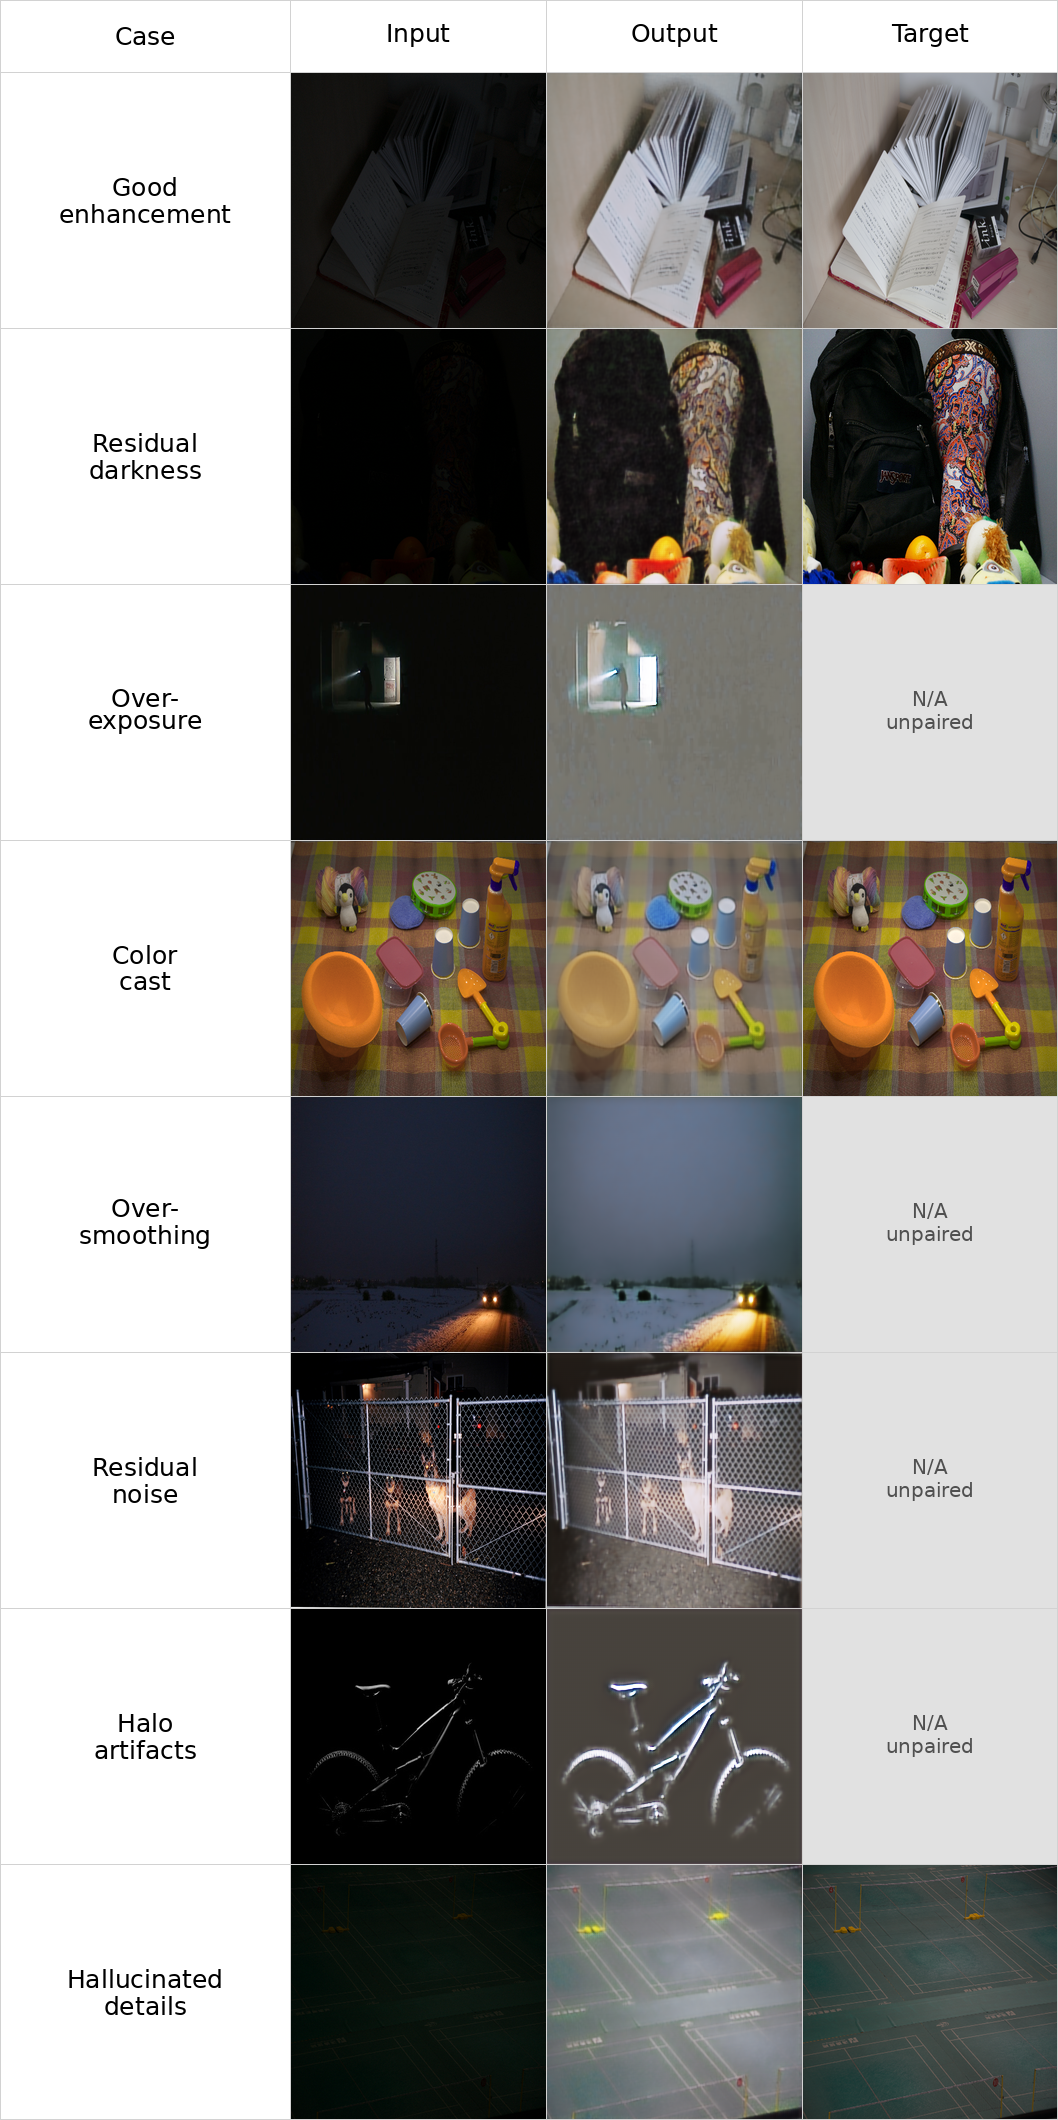
\includegraphics[
	height=\dimexpr\textheight-3\baselineskip\relax,
	keepaspectratio
	]{fig/fac_ecl_qualitative/fac_ecl_qualitative.png}
	\caption{Qualitative examples obtained with the selected FAC-ECL configuration on different datasets used in the project. Each row shows the input, the enhanced output, and the target when available. The rows include one successful enhancement case and representative failure modes: residual darkness, over-exposure, color cast, over-smoothing, residual noise, halo artifacts, and hallucinated details.}
	\label{fig:fac_ecl_qualitative}
\end{figure*}

\analysispar{Successful enhancement}
The first row shows a good enhancement example from LOL-v1. The input image is strongly under-exposed, but the output recovers the open book, the page edges, the text area, and the objects on the right side of the table. The target is not perfectly matched, but the output is close to it in brightness and structure. This example is useful because it shows the intended behavior of FAC-ECL on a compatible LOL-like image: the model increases visibility while keeping the main scene structure and avoiding strong artifacts.

\analysispar{Residual darkness}
The residual darkness example was selected from LOL-v1 because the paired target makes the remaining under-exposure easy to see. The output brightens the scene and makes the patterned object on the right visible, but the black bag on the left remains much darker and less detailed than in the target. This failure shows that FAC-ECL still has difficulty when a region contains very weak input signal. The frequency-aware loss can encourage detail preservation, but it cannot recover information that is almost absent from the low-light input.

\analysispar{Over-exposure}
The over-exposure example was selected from ExDark. The input contains a small bright window or light source inside a mostly dark scene. In the output, that bright region becomes too intense, and the surrounding wall becomes flat and washed out. Since this example is unpaired, no target is available, but the artifact is visually clear. A possible reason is that the model tries to increase the visibility of the dark scene, but the loss does not explicitly penalize local saturation on unpaired data. As a result, small bright regions can still be amplified too much.

\analysispar{Color cast}
The color cast example was selected from MILLs because the paired target makes the chromatic error visible. The output is brighter than the input, but it becomes pale and yellow-green. The orange bowl, the blue object, and the colored toys are less saturated and less natural than in the target. This failure is important because FAC-ECL separates low- and high-frequency content, but it does not include a dedicated color-consistency loss. The model can improve structure and exposure while still shifting the balance between the RGB channels.

\analysispar{Over-smoothing}
The over-smoothing example was selected from ExDark. The output makes the snowy road and the surrounding landscape more visible, but the scene becomes soft and hazy. Fine details in the snow, the distant vegetation, and the road region are weakened. This indicates that the high-frequency term does not completely prevent smooth solutions when the input is dark and low-contrast. A possible reason is that very dark regions contain uncertain high-frequency information, so the model may still prefer a smoother prediction.

\analysispar{Residual noise}
The residual noise example was selected from ExDark because the output still contains visible high-frequency disturbance after enhancement. The fence, the dogs, and the ground become brighter, but the ground and background also show grainy and uneven texture. This failure is different from over-smoothing: here the model preserves or amplifies undesirable high-frequency content. A possible reason is that the high-frequency component used by FAC-ECL contains both real details and sensor noise. Without an explicit denoising constraint, the model may not always distinguish between them.

\analysispar{Halo artifacts}
The halo artifacts example was selected from ExDark because the artifact is very clear around thin structures. The bicycle frame, wheels, and handlebar become surrounded by bright contours. This produces an unnatural outline around the object. This failure suggests that FAC-ECL can still over-enhance strong local transitions. The high-frequency loss encourages local detail, but it does not explicitly enforce edge-aware illumination correction. Therefore, brightness can spread around high-contrast structures and create halos.

\analysispar{Hallucinated details}
The hallucinated details example was selected from LOL-v2 Real because the paired target makes the non-faithful content easy to identify. The output contains bright diagonal haze and repeated line-like patterns over the sports court, while the target is cleaner and more uniform. This is a severe failure because the model is not only changing exposure or color; it is adding visual structure that should not be there. A possible reason is that the input is extremely dark and provides weak evidence for the true scene. In this situation, the model may create plausible-looking patterns while trying to reconstruct missing local information.

\analysispar{Summary}
Overall, the qualitative analysis confirms the quantitative results. FAC-ECL can produce convincing enhancement on close LOL-like images and can improve paired reconstruction on shifted paired data such as MILLs. However, the visual examples show that the method still does not fully control all failure modes. Residual darkness, over-exposure, color cast, over-smoothing, residual noise, halo artifacts, and hallucinated details can still appear, especially when the input is very dark or comes from a different real-world distribution.

\subsection{Mitigation Strategies}

\dots